\section{Arquitectura de la Solución}

\subsection{Visión General de la Arquitectura}

La arquitectura propuesta para el sistema SAT se basa en un enfoque modular y escalable que garantiza la flexibilidad, mantenibilidad y rendimiento del sistema. La solución adopta una arquitectura de microservicios con patrones modernos de desarrollo.

\begin{figure}[h]
\centering
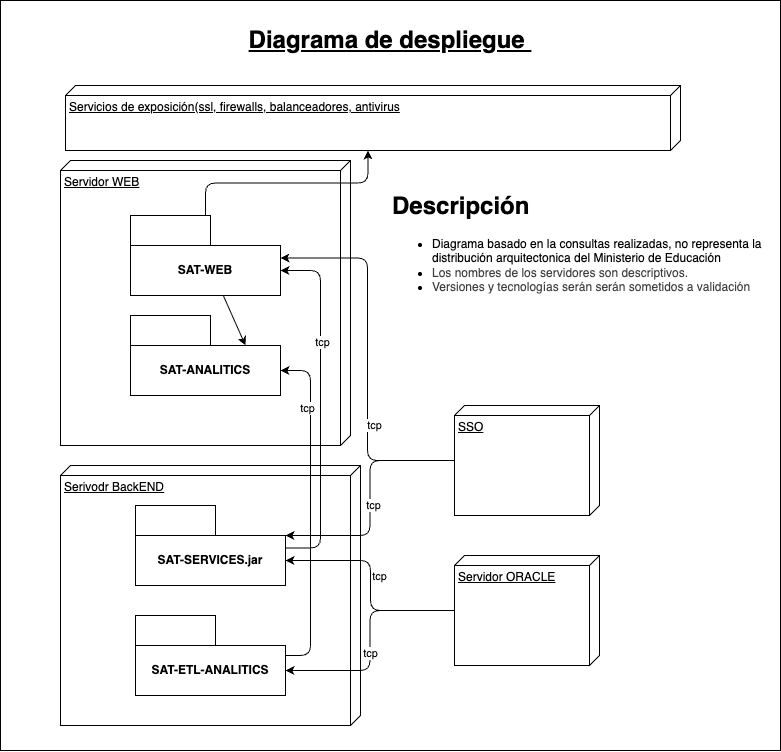
\includegraphics[width=0.8\textwidth]{graficos/arquitectura.png}
\caption{Propuesta de Diagrama de Arquitectura de la Solución SAT}
\label{fig:arquitectura}
\end{figure}

\subsection{Componentes Principales}
En continuidad con los productos existentes expuestos en los terminos de referencia, la arquitectura se compone de los siguientes módulos principales:

\subsection{Capa de exposición}
la capa de exposición es la encargada de interactuar con los usuarios finales y otros sistemas externos. Esta capa está compuesta por las herramientas de frontera como firewalls, balanceadores de carga y API gateways que aseguran la seguridad y el rendimiento del sistema.

\subsubsection{Servidor WEB}
En continuidad con las tecnologias indicadas en los terminos de referencia, las implmementaciones propuestas incluyen:

\begin{itemize}
    \item \textbf{Portal web, SAT-WEB}: Interfaz web para la gestión del sistema, incluyendo configuración, monitoreo y administración de usuarios.
    
    \begin{itemize}
        \item \textbf{Integracion SSO}: Implementar la autenticación única (SSO) utilizando el sistema existente en el Ministerio de Educación, cultura y deporte.
        \item \textbf{Frontend Web}: Aplicación Angular con manejo de autenticación y autorización basado en roles RBAC, con diseño adaptable para tablets y dispositivos móviles.
        \item \textbf{Módulo de usuarios}: Visualización interactiva de datos y alertas en tiempo real, utilizando bibliotecas como D3.js o Chart.js.
        \item \textbf{Modulo de administración}: Implementación de Dashboard interactivo avanzado desarrollado con Streamlit de Python.
        \item \textbf{Módulo de eventos adversos}: Gestión de los eventos adversos.
    \end{itemize}
    \item \textbf{Analitica, SAT-ANALITICS}: El módulo de analitica será el encargado de la presentación de los datos analizados, generando reportes y visualizaciones para la toma de decisiones. 
    Fundamentalmente estará compuesto por:
        \begin{itemize}
            \item \textbf{Análisis}: Creación de reportes personalizados en formatos PDF y Excel, utilizando bibliotecas como JasperReports o Apache POI.
            \item \textbf{Reportes}: Gráficos y tablas interactivas para el análisis de tendencias y patrones, integrándose con herramientas de BI como Power BI o Tableau.
        \end{itemize}
\end{itemize}

\subsubsection{Capa de Servicios}
\begin{itemize}
    \item \textbf{SAT-SERVICES}: Punto de entrada único para todas las solicitudes basadas en servicios RESTful, gestionando la seguridad y el enrutamiento, documentación con Swagger.\\
    Producto construido con Java Spring Boot, con arquitectura de microservicios, basado en arquitectura hexagonal, con integración a diferentes fuentes de datos.
    \begin{itemize}
        \item \textbf{Módulo de Gestión de Usuarios}: Manejo de autenticación y autorización basado en roles RBAC, integrándose con el sistema SSO existente.
        \item \textbf{Módulo de Eventos Adversos}: Gestión de los eventos adversos, incluyendo la detección, notificación y análisis de incidentes.
        \item \textbf{Módulo de Configuración}: Gestión de parámetros del sistema, incluyendo umbrales de alerta, reglas de negocio y configuraciones específicas del cliente.
        \item \textbf{Módulo de Auditoria}: Registro y seguimiento de todas las acciones realizadas en el sistema, garantizando la trazabilidad y cumplimiento normativo.
        \item \textbf{Módulo de Notificaciones}: Gestión del envío de alertas y notificaciones a través de diferentes canales (correo electrónico, SMS, etc.).
    \end{itemize}
    \item \textbf{SAT-ETL-ANALITICS}: Paquete encargado de la extracción, transformación y carga de datos para el módulo de analítica, desarrollado en python, implementando un pipeline encargado de la generación de una base de datos de análisis.
\end{itemize}

\subsubsection{SSO}
Sistema de autenticación única (SSO) existente en el Ministerio de Educación, cultura y deporte, utilizando protocolos estándar como OAuth2 o SAML para garantizar la seguridad y facilidad de acceso a los usuarios autorizados.

\subsubsection{SMTP}
Sistema de gestión de correo electrónico que permite el envío y recepción de correos electrónicos

\subsubsection{ORACLE}
Sistema de gestión de bases de datos relacional que permite el almacenamiento y recuperación de datos de manera eficiente y segura.

\subsection{Tecnologías Propuestas}
En continuidad de las tecnologias indicadas en los terminos de referencia, se propone el siguiente stack tecnológico:

\begin{table}[h]
\centering
\begin{tabular}{|l|l|}
\hline
\textbf{Componente} & \textbf{Tecnología} \\
\hline
Backend & Java Springm, JPA, smpt,  \\
\hline
Frontend & Angular, chart.js, primereact\\
\hline
Frontend analitics & Streamlit \\
\hline
Base de Datos transaccional & ORACLE \\
\hline
Base de Datos analitica & DUCKDB \\
\hline
\end{tabular}
\caption{Stack Tecnológico Propuesto}
\label{tab:stack_tecnologico}
\end{table}

\subsection{Versionamiento y Despliegue}

Para el desarrollo de la solución se utilizará git como herramienta de versionamiento, teniendo ramas de desarrollo, pruebas, piloto y producción.

El método de despliegue será ajustado a los métodos actuales del Ministerio de Educación, cultura y deporte, asegurando una integración fluida con los sistemas existentes, de no existir una método establecido, se propone la implementación de pipelines de CI/CD utilizando GitLab CI para automatizar pruebas y despliegues.